\documentclass[a4paper, 12pt]{article}

\usepackage[english,russian]{babel}
\usepackage[T2A]{fontenc}
\usepackage[utf8]{inputenc}
\usepackage{geometry}
\usepackage{enumitem}
\usepackage{setspace}
\usepackage{amssymb}
\usepackage{graphicx}
\usepackage{wrapfig}
\usepackage{float}
\usepackage{amsmath}
\usepackage{textcomp}
\usepackage{dsfont}

\geometry{top=5mm, left=1cm}
%\setlength{\parindent}{0}
\renewcommand{\arraystretch}{1.2}
\linespread{1}

\begin{document}
    \begin{center}
        \textbf{Сферическая геометрия №2}\\
        Прямые, полюсы, поляры
    \end{center}

    \begin{center}
        \textbf{№1}
    \end{center}

    Докажите, что если плоскость проходит через центр сферы, то она содержит ее диаметр.

    \textbf{Решение}\\

    1) Если плоскость проходит через центр сферы, то расстояние от центра сферы до плоскости равно нулю.
    Тогда радиус полученной в сечении окружности равен радиусу сферы, а значит любой диаметр окружности является диаметром сферы.

    \begin{center}
        \textbf{№2}
    \end{center}

    Докажите, что прямой на сфере соответствует единственная пара полюсов.

    \textbf{Решение}\\

    Предположим, что существует две пары полюсов, тогда из центра сферы восстановлены два перпендикуляра к плоскости сечения,
    что противоречит теореме о единственности перпендикуляра, проведенного из точки к плоскости.\\

    Таким образом, существует не более 1 пары полюсов, соответствующих прямой на сфере.\\

    Существование следует из той же теоремы о прямой, перпендикулярной к плоскости

    \begin{center}
        \textbf{№3}
    \end{center}

    Докажите, что двум диаметрально противоположным точкам на сфере соответствует единственная поляра.

    \textbf{Решение}\\

    Предположим, что это не так, тогда через центр проходит две плоскости, перпендикулярные к диаметру, проходящему через полюсы.
    Тогда такие плоскости параллельны по теореме о плоскостях перпендикулярных к одной прямой,
    а так как они имеют общую точку центр сферы, то они совпадают.

    \begin{center}
        \textbf{№4}
    \end{center}

    Докажите, что cуществует единственная прямая, проходящая через две данные различные точки,
    кроме случая, когда эти точки диаметрально противоположны;
    тогда таких прямых бесконечно много.

    \textbf{Решение}\\

    1) Точки не диаметрально противоположные.
    В этом случае можно воспользоваться аксиомой стереометрии и рассмотреть три точки: два полюса и центр сферы.
    Тогда эти точки не лежат на одной прямой, а значит задают единственную плоскость.
    Любая плоскость, содержащая центр сферы будет высекать большую окружность(и наоборот), то есть являться прямой на сфере,
    единственность следует из замечания выше.

    2) Если точки диаметрально противоположные, то они лежат на диаметре, то есть центр сферы и полюсы лежат на одной прямой,
    тогда через эту прямую можно провести бесконечное количество плоскостей, которые будут содержать диаметр, а значит
    высекать большую окружность, что соответствует определению прямой на сфере.

    \begin{center}
        \textbf{№5}
    \end{center}

    Точки $A$ и $C$ - полярно сопряженные на окружности радиуса $R$.
    Найдите Евклидово расстояние между этими точками.

    \textbf{Решение}\\

    \begin{center}
        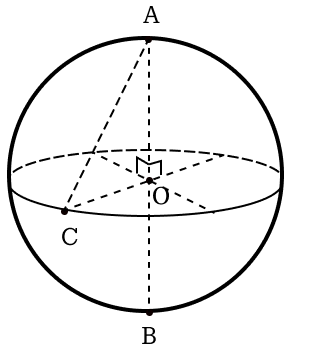
\includegraphics[width=0.2\textwidth]{images/img2}\\
    \end{center}

    Для определенности будем считать, что точка $A$ - полюс, а точка $C$ лежит на поляре полюса.\\

    Так как поляра является большой окружностью, то ее радиус равен радиусу сферы, а так как $AB$ - перпендикуляр,
    то по теореме Пифагора получаем:
    \[
        AC = \sqrt {CO ^ 2 + AO ^ 2} = \sqrt {R ^ 2 + R ^ 2} = R\sqrt {2}
    \]

    Ответ: $R\sqrt{2}$


    \begin{center}
        \textbf{№6}
    \end{center}

    Евклидово расстояние между двумя полярно сопряженными точками равно 12 см.
    Чему равна длина прямой на сфере?

    \textbf{Решение}\\

    Евклидово расстояние между полярно сопряженными точками равно $R\sqrt{2}$, где $R$ - радиус сферы, тогда
    если Евклидово расстояние рано $12\sqrt{2}$, то $R = 12$ и длинна прямой равна:
    \[ L = 2\pi R = 24\pi\]

    Ответ: $24\pi$

    \begin{center}
        \textbf{№7}
    \end{center}

    Угол между двумя секущими плоскостями, проходящими через центр сферы, равен $\alpha$.
    Чему равен угол между двумя прямыми,
    каждая из которых соединяет полюсы соответсвующий плоскостей?

    \textbf{Решение}\\

    \begin{center}
        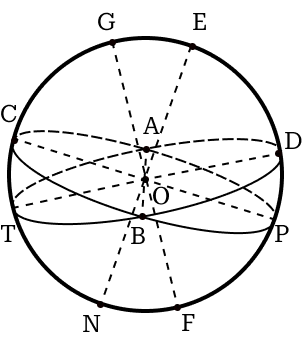
\includegraphics[width=0.2\textwidth]{images/img3} \quad
        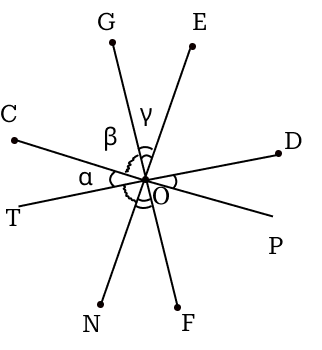
\includegraphics[width=0.2\textwidth]{images/img4}\\
    \end{center}

    1) Так как секущие прямые имеют общую точку, то они пересекаются по прямой $AB$, что следует из аксиом стереометрии.

    2) Восстановим перпендикуляр $OC\bot AB$ в плоскости $(BOC)$ и перпендикуляр $OD \bot AB$ в плоскости $BOD$.
    Проведем прямые, соединяющие полюсы $GF$ и $EN$, так как прямая $AB$ лежит в плоскостях сечений,
    то $CF \bot AB$ и $EN \bot AB$.

    3) $OC \bot AB$, $OD \bot AB$, $GF \bot AB$, $EN \bot AB$,
    тогда эти прямые ($OC, OD, GF, EN$) лежат в плоскости $(COE)$, перпендикулярной прямой $AB$.

    4) Вынесем планиметрический чертеж, на котором $\angle COT = \alpha$ - линейный угол двугранного угла $CABT$,
    который равен углу между секущими плоскостями.
    Так как $GF \bot (TOA)$, то $GF \bot TD \subset (TOA)$ и так как $EN \bot (COP)$, то $EN \bot CP \subset (COP)$.
    Получаем, что $\beta = 90^\circ - \alpha = \angle COT$

    5) Таким образом:
    \[
        2\beta + \alpha + \gamma = 180^{\circ}
    \]
    \[
        180^{\circ} - 2\alpha + \alpha + \gamma = 180 ^{\circ}
    \]
    \[ \alpha = \gamma \]

    Ответ: $\alpha$

    \begin{center}
        \textbf{№8}
    \end{center}

    При каком условии две прямые на сфере содержат полюсы друг друга?

    \textbf{Решение}\\

    Так как плоскости содержат полюсы друг друга, то они содержат перпендикуляры друг друга,
    что по признаку перпендикулярности плоскостей означает перпендикулярность плоскостей.

    Ответ: при условии перпендикулярности плоскостей, задающих прямые на сфере.

    \begin{center}
        \textbf{№9}
    \end{center}

    Угол между секущими плоскостями, проходящими через центр сферы равен $\alpha$, радиус сферы равен $R$.
    Найдите Евклидово расстояние между всеми полюсами.

    \textbf{Решение}\\

    1) Из задачи 7 знаем, что угол между секущими плоскостями равен углу между диаметрами, соединяющими их полюсы,
    тогда справедлив следующий планиметрический чертёж.

    \begin{center}
        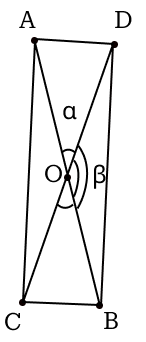
\includegraphics[width=0.1\textwidth]{images/img5}\\
    \end{center}

    2) Причем $AO = OB = CO = OD = R$, тогда применяя теорему косинусов получим:
    \[  \begin{cases}
            CB ^ 2 = AD ^ 2 = AO ^ 2 + DO ^ 2 - 2 AO * DO *\cos \alpha\\
            AC ^ 2 = BD ^ 2 = AO ^ 2 + CO ^ 2 - 2AO * CO * \cos \beta
    \end{cases}
    \rightarrow
    \]
    \[
        \begin{cases}
            CB ^{ 2}  = 2R^2 - 2R^2\cos \alpha\\
            AC ^2 = 2R^2 - 2R^2\cos \beta
        \end{cases}
        \rightarrow
        \begin{cases}
            CB  = R\sqrt{2 - 2\cos \alpha}\\
            AC = R\sqrt{2 - 2\cos \beta}
        \end{cases}
        \rightarrow
        \begin{cases}
            CB  = R\sqrt{2 - 2\cos \alpha}\\
            AC = R\sqrt{2 - 2\cos (\pi - \alpha)}
        \end{cases}
        \rightarrow
    \]
    \[
        \begin{cases}
            CB  = R\sqrt{2 - 2\cos \alpha}\\
            AC = R\sqrt{2 + 2\cos \alpha}
        \end{cases}
    \]
    \\

    3) $A$ и $B$, $C$ и $D$ лежат на диаметре, поэтому $AB = CD = 2R$. \\

    Ответ: $AD = CB = R\sqrt {2 - 2\cos \alpha}$; $AC = DB = R\sqrt {2 + 2\cos \alpha}$; $AB = CD = 2R$.
    \begin{center}
        \textbf{№10}
    \end{center}

    Чему равна площадь треугольника, образованного двумя полисами и полярно сопряженной с ними точкой,
    если радиус сферы $R$.

    \textbf{Решение}\\

    \begin{center}
        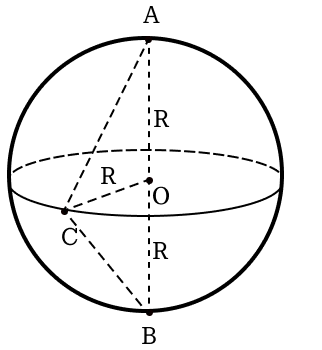
\includegraphics[width=0.2\textwidth]{images/img6}\\
    \end{center}

    1) $AB \bot CO$ по определению полюсов.\\

    2)\[
          S_{\triangle ABC} = \frac{1}{2} CO * AB = \frac{1}{2} R * 2R = R ^ 2
    \]

    Ответ: $R ^ 2$
    \begin{center}
        \textbf{№11}
    \end{center}

    Угол между двумя секущими плоскостями равен $\alpha$.
    Чему равен угол между диаметром, соединяющим одну пару полюсов одной плоскости, и другой плоскостью?

    \textbf{Решение}\\

    Исходя из задач 7 и 9 получаем следующий планиметрический чертёж:

    \begin{center}
        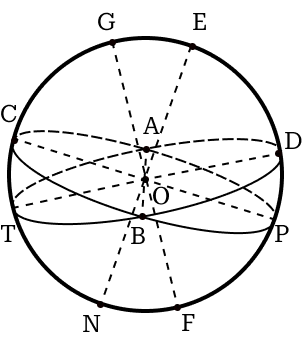
\includegraphics[width=0.2\textwidth]{images/img7} \quad
        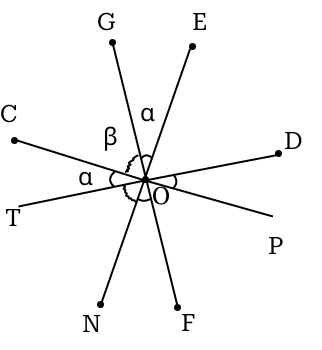
\includegraphics[width=0.2\textwidth]{images/img8}\\
    \end{center}

    1) Необходимо найти угол $\beta$, так как если из $G$ опустить перпендикуляр к $CP$, то он будет перпендикулярен
    плоскости сечения, так как будет перпендикулярен двум пересекающимся прямым $AB$ и $CP$.

    2) $\beta = 90^\circ - \alpha$

    Ответ: $90^\circ - \alpha$

    \begin{center}
        \textbf{№12}
    \end{center}

    Длина большой окружности равно L, радиус сферы R.
    На большой окружности выбраны две точки, расстояние между которыми h.
    Найдите периметр и площадь треугольника,
    составленного из этих точек окружности и полярно сопряженной с ними точкой сферы.

    \textbf{Решение}\\

    \begin{center}
        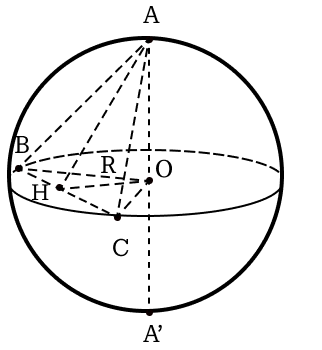
\includegraphics[width=0.2\textwidth]{images/img9}\\
    \end{center}

    1) $BO = CO = AO = R$, $BC = h$

    2) $L = 2\pi R\rightarrow R = \frac{L}{2\pi}$

    3) По теореме Пифагора:
    \[
        AB = \sqrt {BO ^ 2 + AO ^ 2} = \sqrt {2R^2} = R\sqrt {2} = \frac{L}{2\pi}\sqrt {2} = AC
    \]

    4) Проведем $AH \bot BC$, тогда $OH \bot BC$, так как $\triangle BOC$ - равнобедренный.

    5) По теореме Пифагора:
    \[
        OH = \sqrt {OC ^ 2 - HC ^ 2} = \sqrt {R ^ 2 - \frac{h ^ 2}{4}}
    \]
    \[
        AH = \sqrt {OH ^ 2 + AO ^ 2} = \sqrt {R ^ 2 - \frac{h ^ 2}{4} + R ^ 2} = \sqrt {2R^2 - \frac{h ^ 2}{4}}
    \]

    6) Таким образом,
    \[
        P_{\triangle ABC} = AB + AC + BC = 2\frac{L}{2\pi}\sqrt {2} + h = \frac{L}{\pi}\sqrt {2} + h
    \]
    \[
        S_{\triangle ABC} = \frac{1}{2} BC * AH = \frac{1}{2} h * \sqrt {2R^2 - \frac{h ^ 2}{4}}
    \]


\end{document}
